\section{Research Plan}

\subsection{Overview}

\begin{figure}[t]
\centering
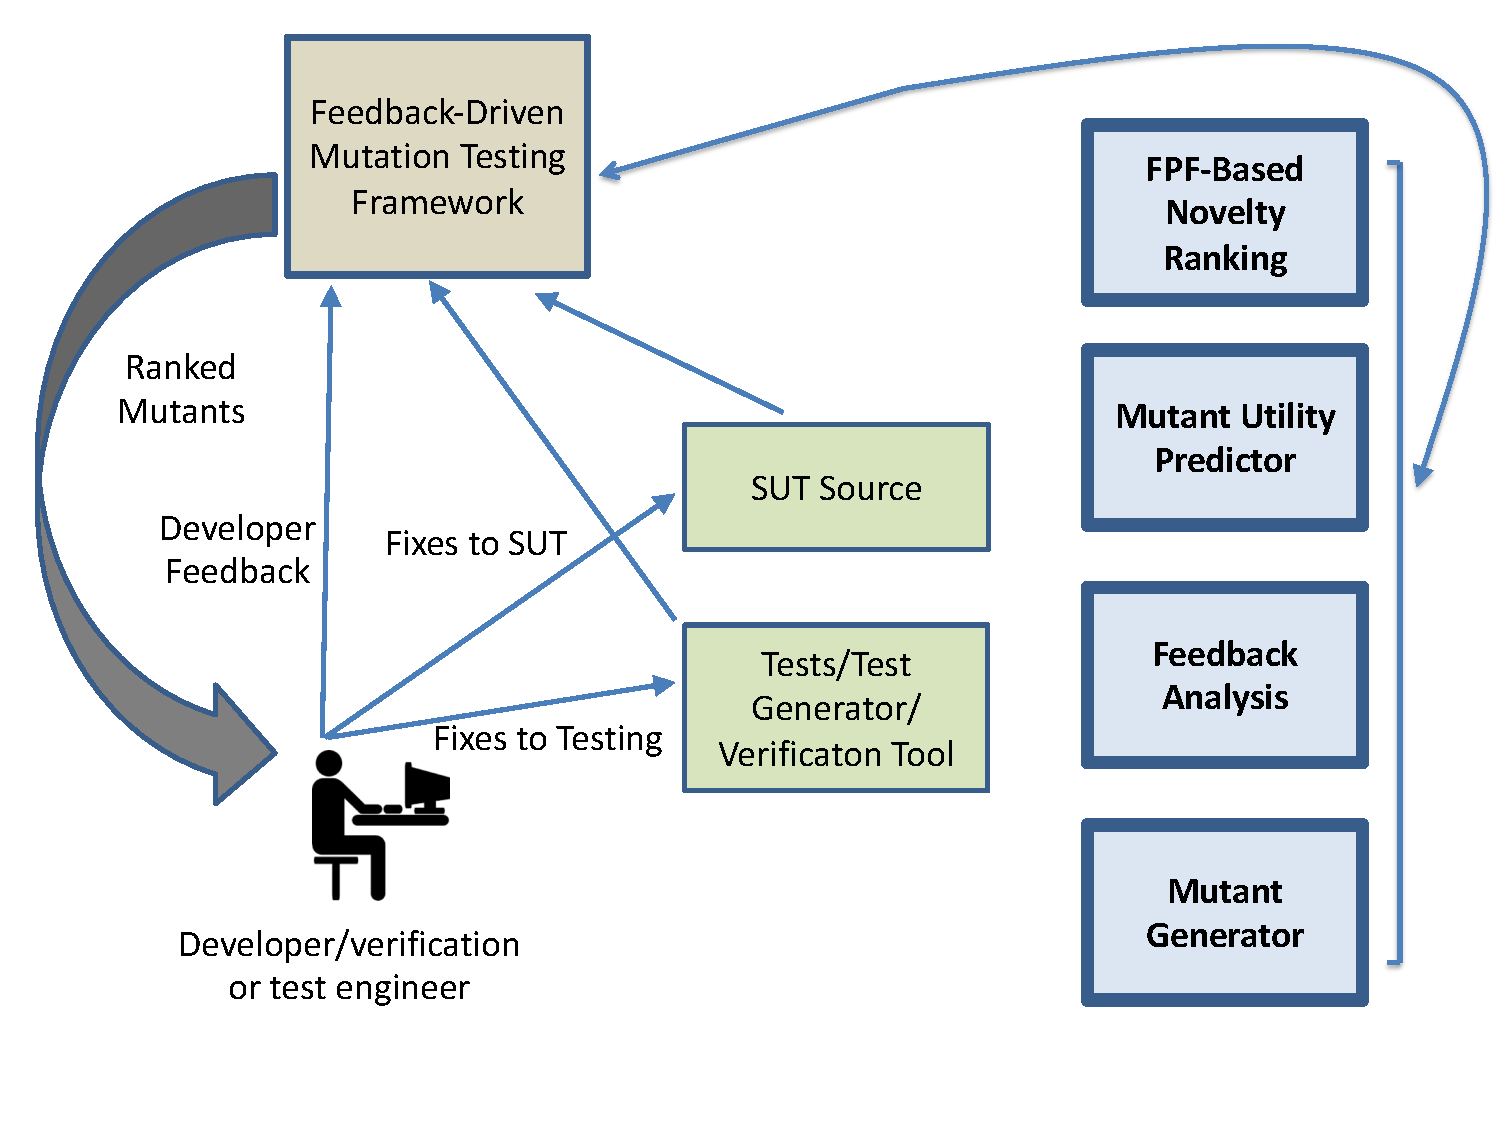
\includegraphics[width=0.8\columnwidth]{TestFlow}

\caption{Basic flow of feedback-driven mutation testing.}
\label{fig:flow}
\end{figure}

Figure \ref{fig:flow} shows the basic outline of a proposed workflow
and components needed to support feedback-driven mutation testing.

\subsubsection{FPF-Based Novelty Ranking}
\label{sec:fpfplan}

\subsubsection{Mutant Utility Predictor}

\subsubsection{Feedback Analysis}

\subsubsection{Mutant Generator}

\subsection{Core Research Questions}

\subsubsection{Research Questions for Feedback-Driven Mutation Testing
in General}

\begin{enumerate}
\item How can we form a generalized, language-agnostic representation
  of and distance metric for program mutants for use in FPF?
\item How can we incorporate feedback from users into the
  representation and distance metric?
\item How can we set budgets for automated test generation and
  timeouts for verification efforts to quickly estimate whether a
  mutant is killable?
\item How can we most effectively use already generated killing tests
  and counterexamples to prune mutants?
\item Is distance-based clustering plus timing information useful for quickly
  eliminating killable mutants similar to already-killed mutants?  How
  does this relate to Predictive Mutation Testing (PMT)?
\item How can we balance FPF-based selection of mutants for novelty
  with predictions of mutant equivalence, outcome, dominance, and
  productivity?
\item How can we identify outliers in otherwise similar groups of
  mutants, and is such identification useful?
\item Can we predict whether a mutant's unkillability is due to poor test
  generation  or due to oracle weakness?
\end{enumerate}

\subsubsection{Research Questions Specific to Any-Language Mutation}

\begin{enumerate}
\item How can we maximize the efficiency and usability of a
  fundamentally language-agnostic regular-expression-based approach to
  mutant generation?
\item How can we extend the language of regular expressions to allow
  for language-agnostic definition of mutation operators that require
  more parsing-like analysis of code structure, without compromising
  the usability and simplicity of the approach?
\item Is it possible to perform on-the-fly mutant generation for very
  large projects, and reconcile this approach with FPF (e.g., generate
  new mutants with, possibly approximate, desired distances from
  already evaluated mutants)?
\end{enumerate}

\subsection{Work and Evaluation Plans}
\label{sec:workplan}
\subsection{Evaluation Plan}
